\chapter[Protótipos]{Protótipos}

\section{Baixa Fidelidade}

Os protótipos de baixa fidelidade foram concebidos durante a fase inicial do projeto. Desenhados à mão utilizando lápis, borracha e papel, foram feitas representações de maneira rápida e superficial, apenas margeando a ideia do projeto e definindo inicialmente sua interação com o usuário, não se preocupando tanto com elementos de layout, cores, disposições, etc.

\textbf{Telas:}

\begin{figure}[H]
	\begin{center}
		\includegraphics[keepaspectratio,scale=0.15]{figuras/prototipo_de_papel.eps}
		\caption{Protótipo de Baixa Fidelidade}
	\end{center}
\end{figure}

\section{Média Fidelidade}

Os protótipos de média fidelidade foram desenvolvidos apos a aplicação dos testes com os protótipos de baixa fidelidade. Utilizamos o softwares de prototipação Balsamiq para auxilio na apresentação da estrutura e o conteúdo da interface, definindo peso, relevância e relação dos elementos, formando o layout básico do projeto.

\textbf{Telas:}

\begin{figure}[H]
	\begin{center}
		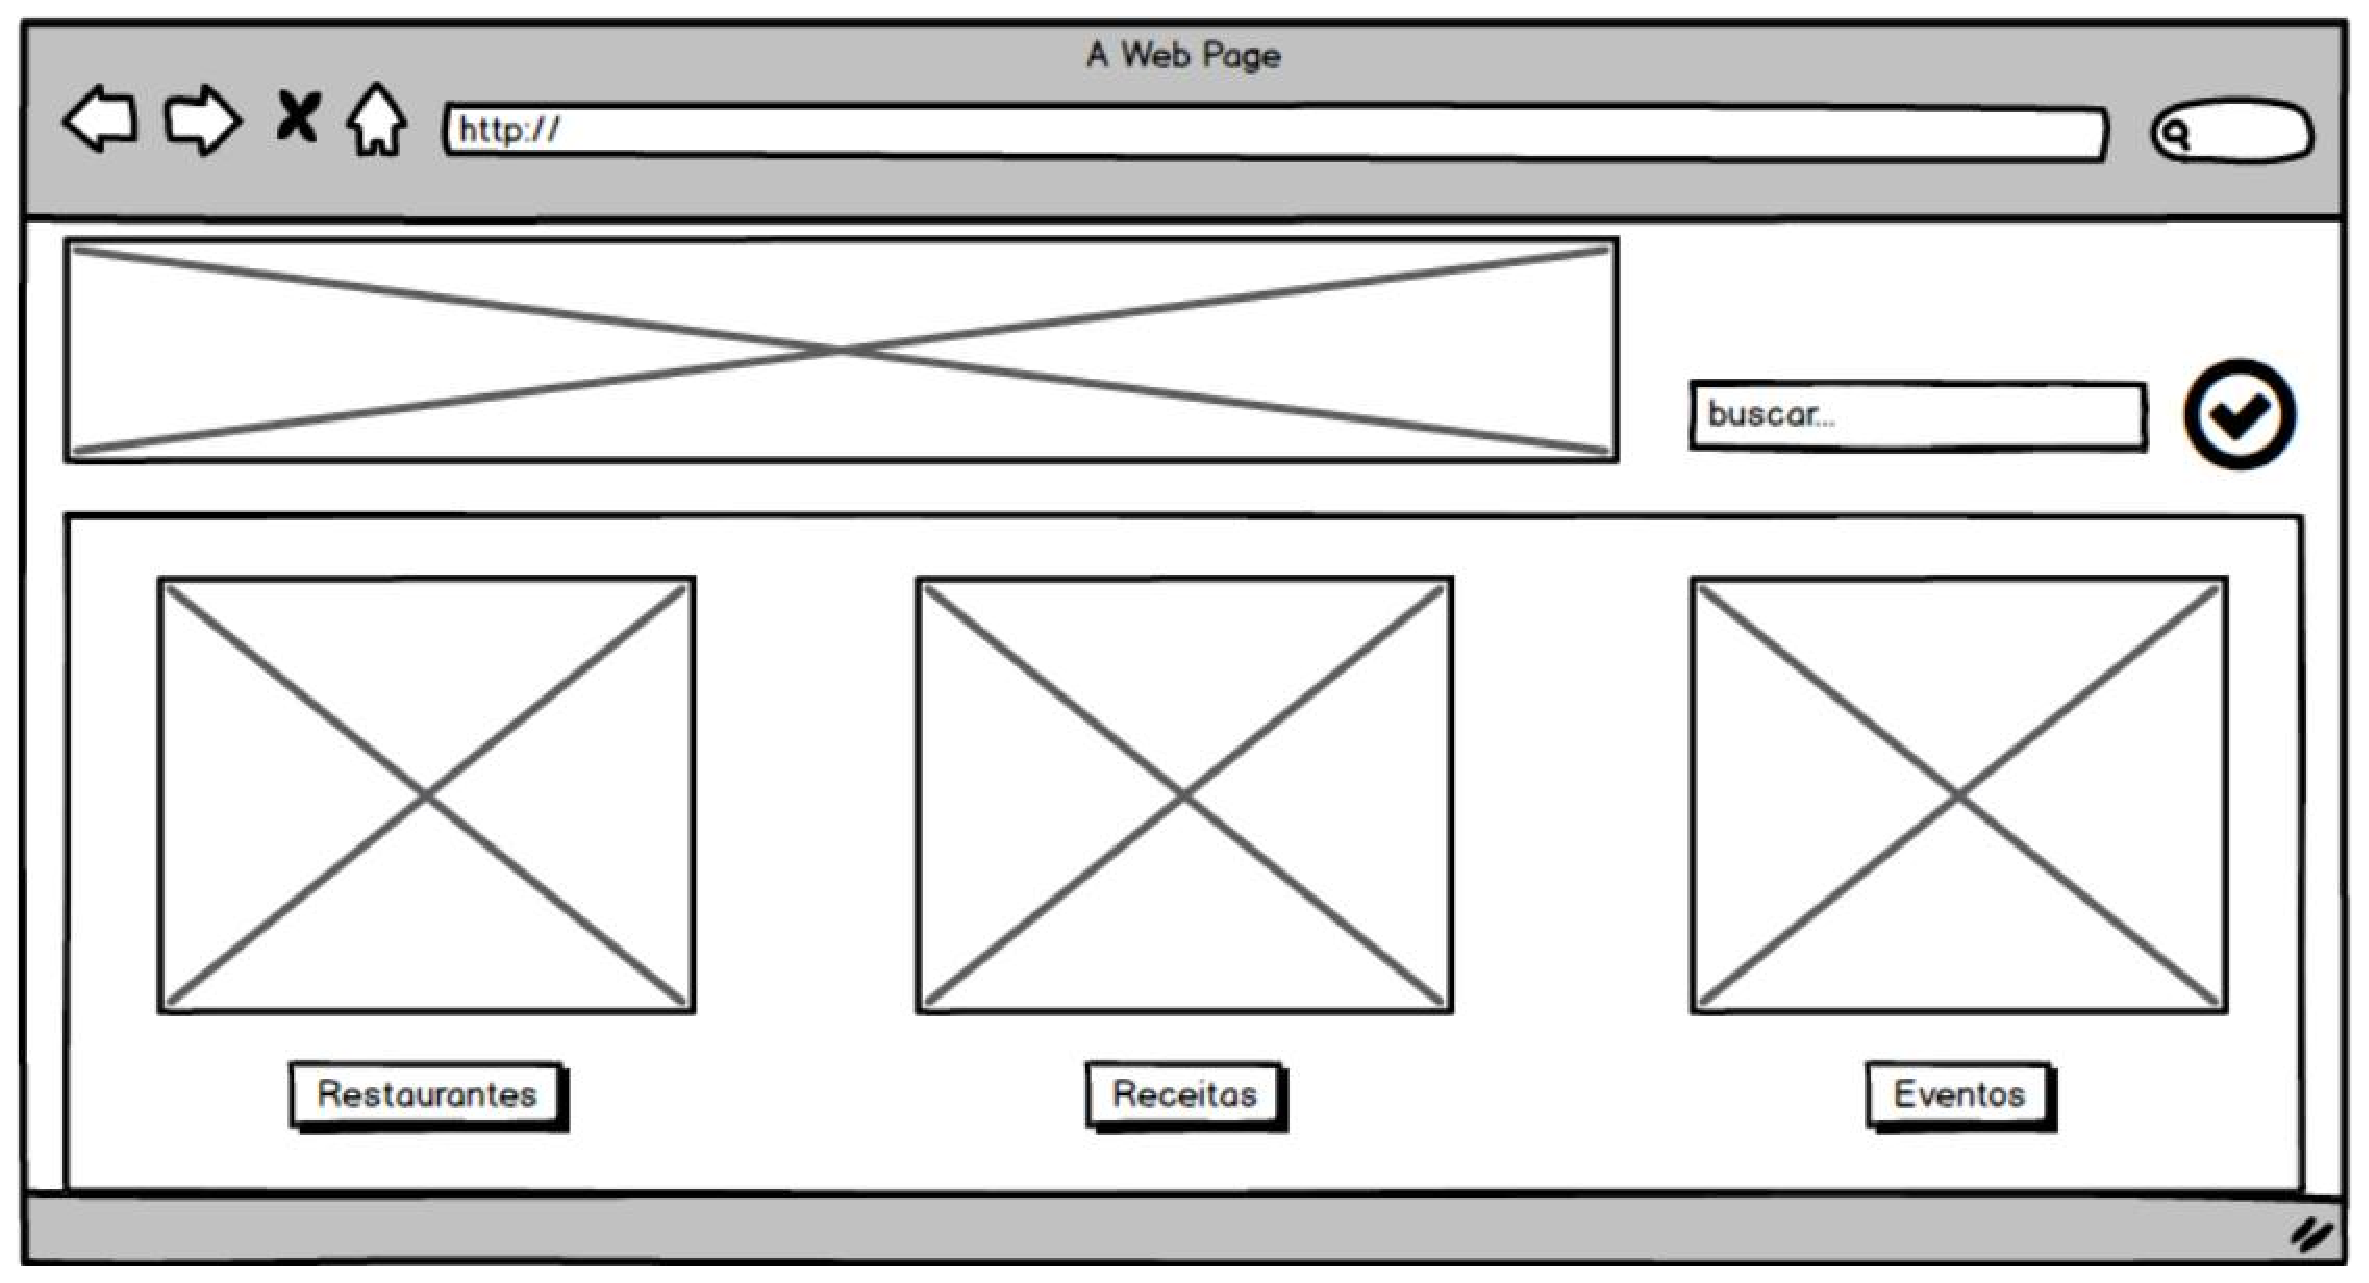
\includegraphics[keepaspectratio,scale=0.3]{figuras/media_fidelidade/prototipo1.eps}
		\caption{Protótipo Média Fidelidade}
	\end{center}
\end{figure}

\begin{figure}[H]
	\begin{center}
		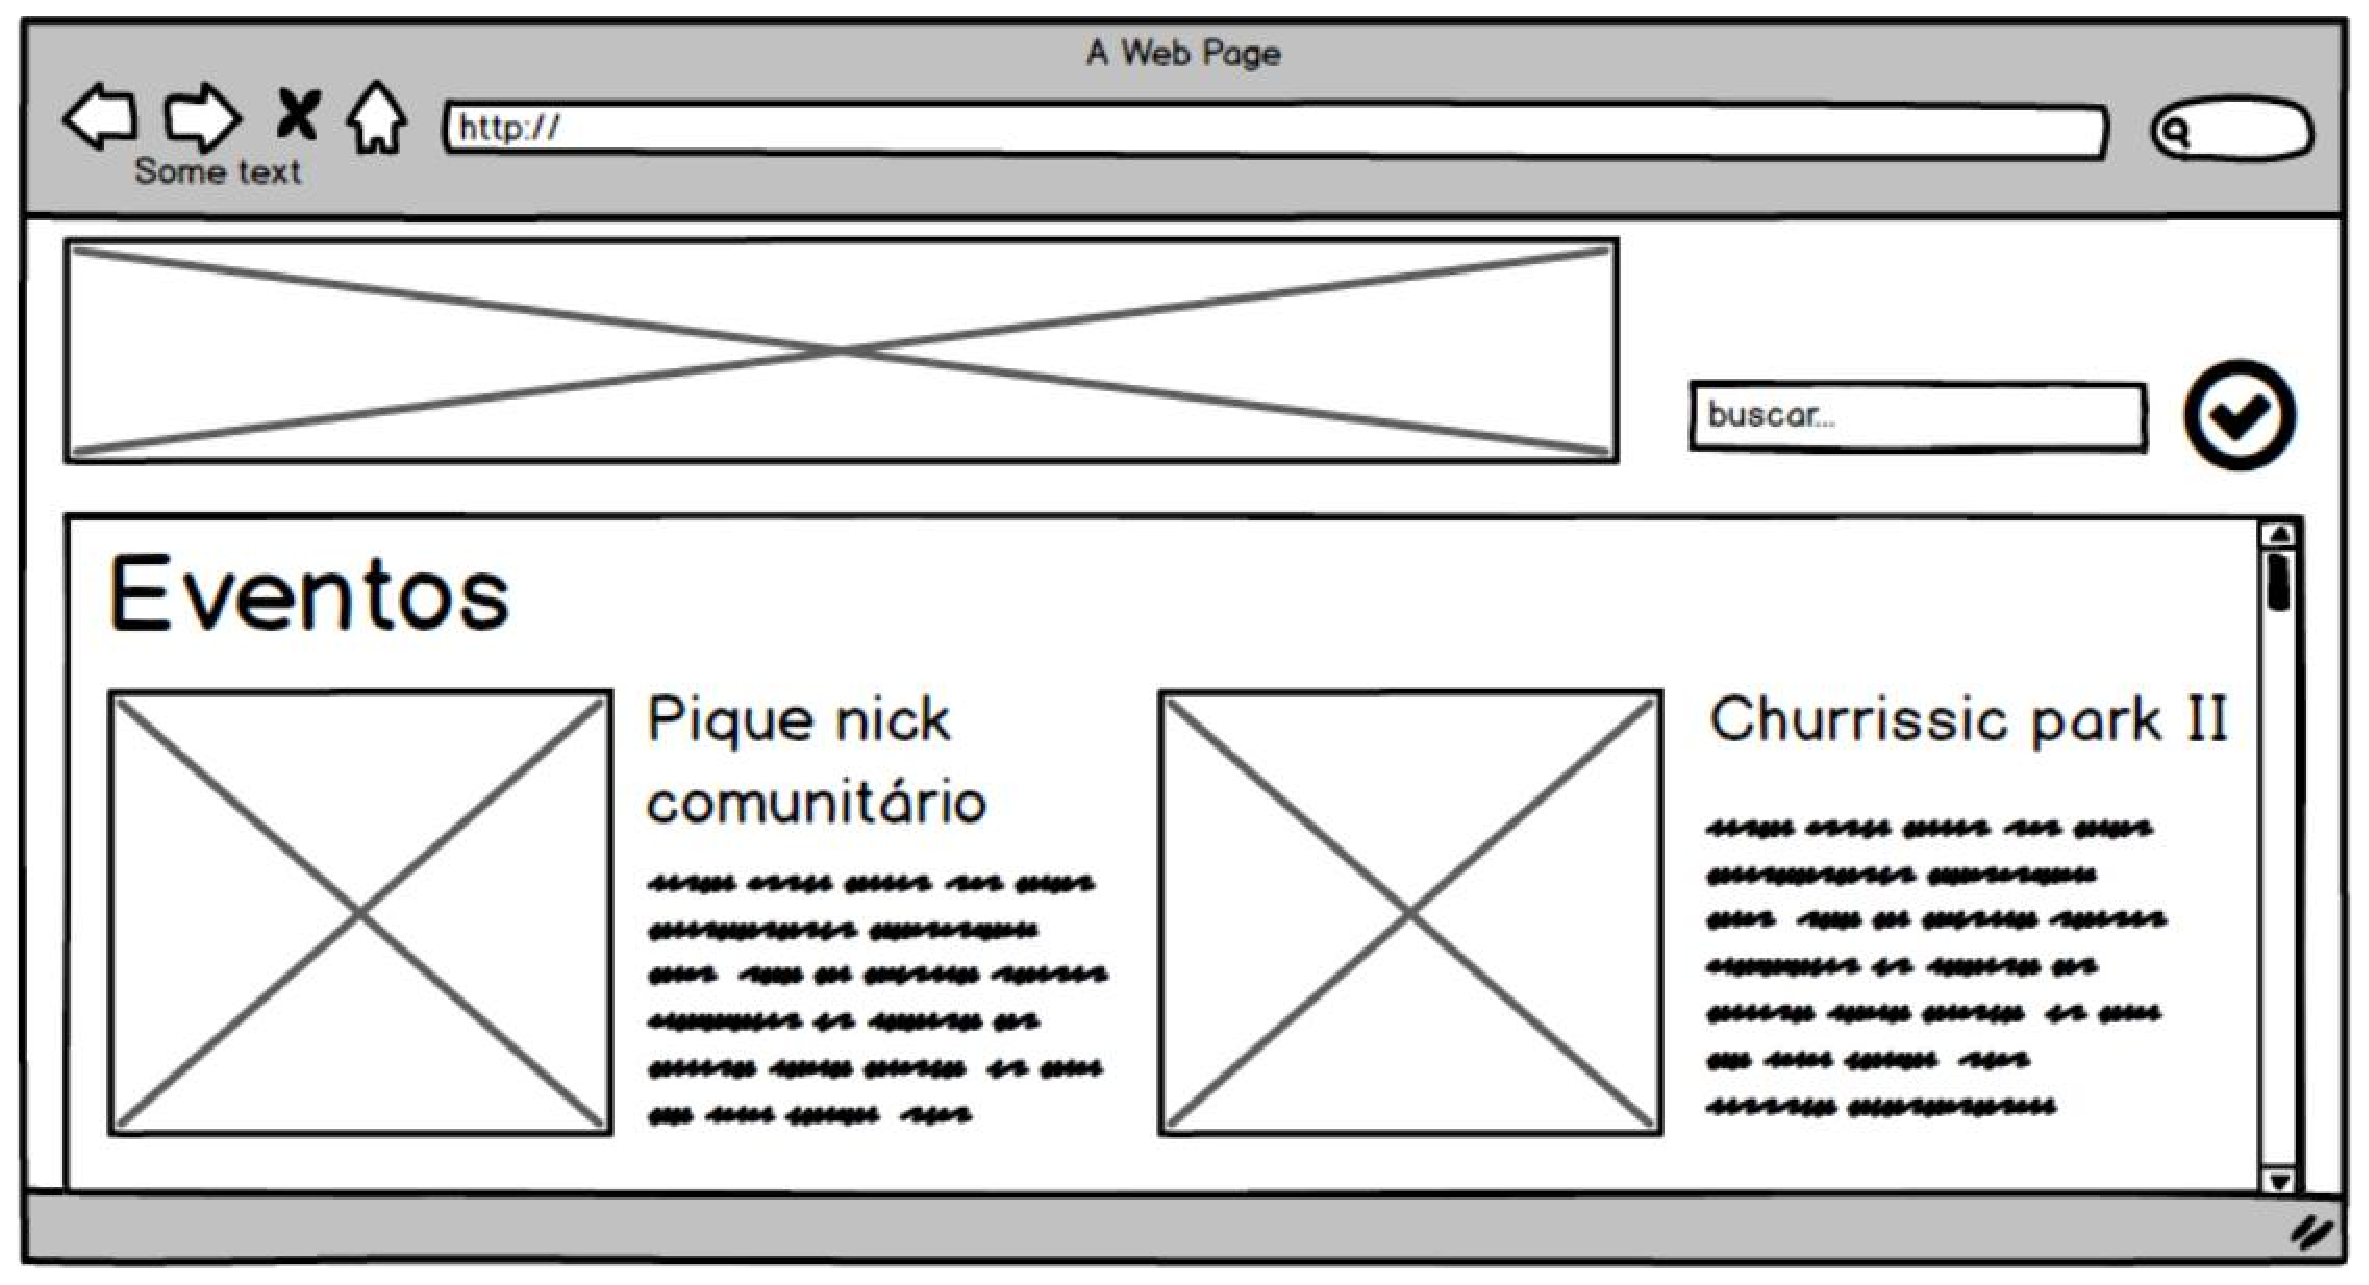
\includegraphics[keepaspectratio,scale=0.3]{figuras/media_fidelidade/prototipo2.eps}
		\caption{Protótipo Média Fidelidade}
	\end{center}
\end{figure}

\begin{figure}[H]
	\begin{center}
		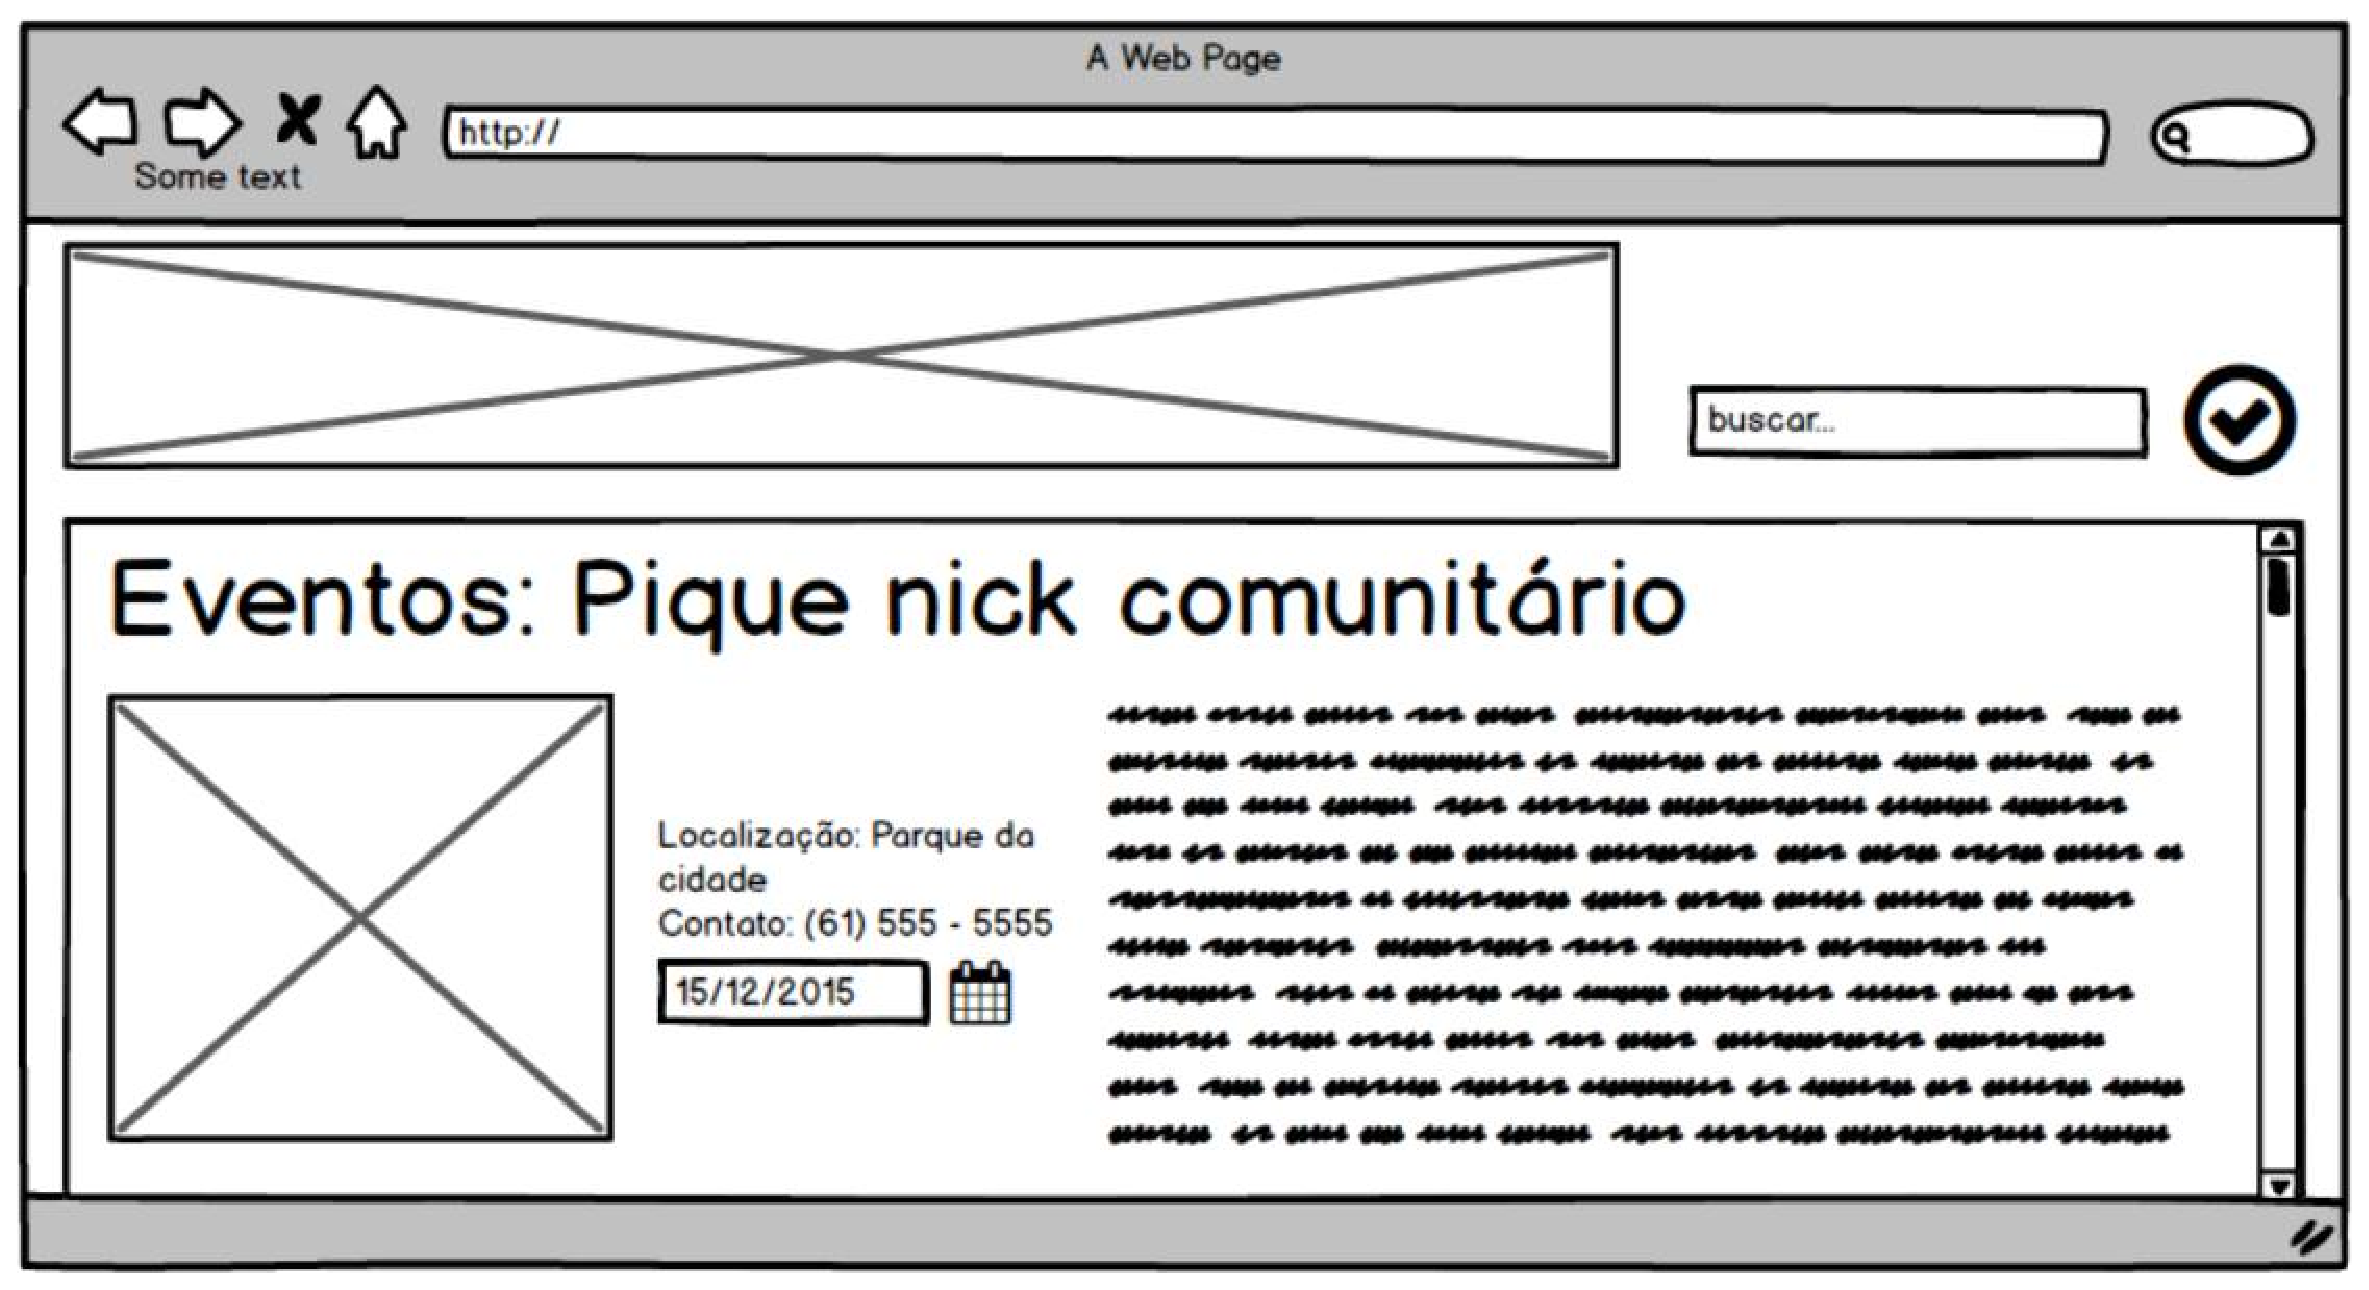
\includegraphics[keepaspectratio,scale=0.3]{figuras/media_fidelidade/prototipo3.eps}
		\caption{Protótipo Média Fidelidade}
	\end{center}
\end{figure}

\begin{figure}[H]
	\begin{center}
		\includegraphics[keepaspectratio,scale=0.3]{figuras/media_fidelidade/prototipo4.eps}
		\caption{Protótipo Média Fidelidade}
	\end{center}
\end{figure}

\begin{figure}[H]
	\begin{center}
		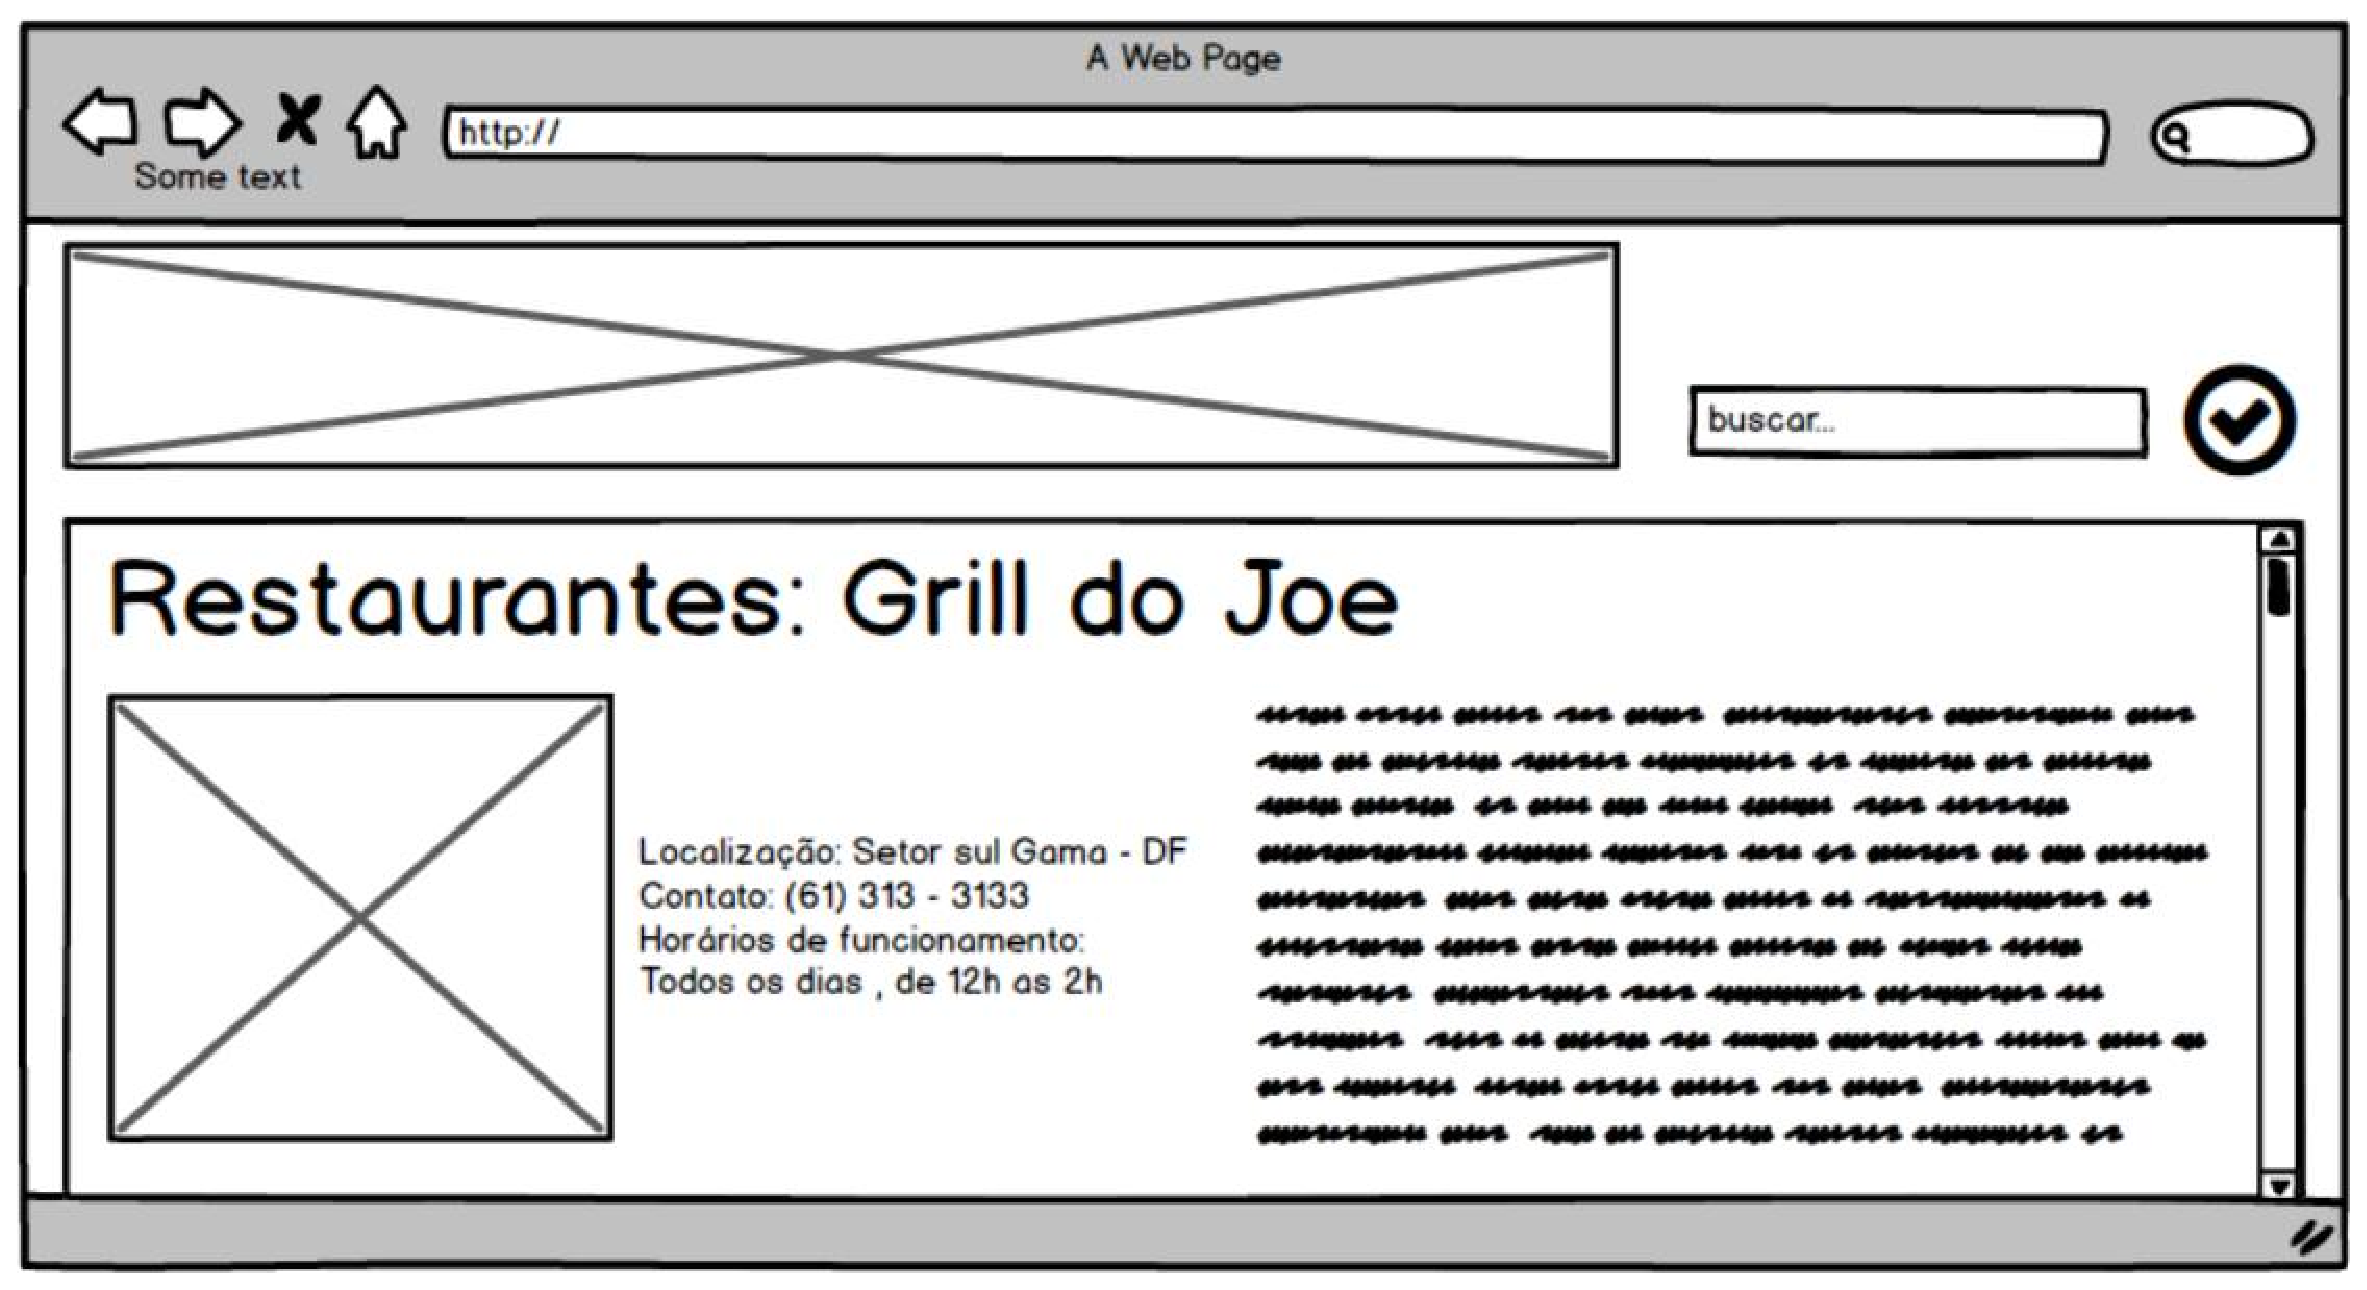
\includegraphics[keepaspectratio,scale=0.3]{figuras/media_fidelidade/prototipo5.eps}
		\caption{Protótipo Média Fidelidade}
	\end{center}
\end{figure}

\begin{figure}[H]
	\begin{center}
		\includegraphics[keepaspectratio,scale=0.3]{figuras/media_fidelidade/prototipo6.eps}
		\caption{Protótipo Média Fidelidade}
	\end{center}
\end{figure}

\begin{figure}[H]
	\begin{center}
		\includegraphics[keepaspectratio,scale=0.3]{figuras/media_fidelidade/prototipo7.eps}
		\caption{Protótipo Média Fidelidade}
	\end{center}
\end{figure}




\section{Alta Fidelidade}

Os protótipos funcionais constituem a representação mais próxima do sistema que será desenvolvido. Nele é possível simular o fluxo completo das funcionalidades, permitindo a interação do usuário como se fosse o sistema final. A aparência visual, as formas de navegação e interatividade já são concebidas e aplicadas aos protótipos de alta fidelidade.

\textbf{Telas:}

\begin{figure}[H]
	\begin{center}
		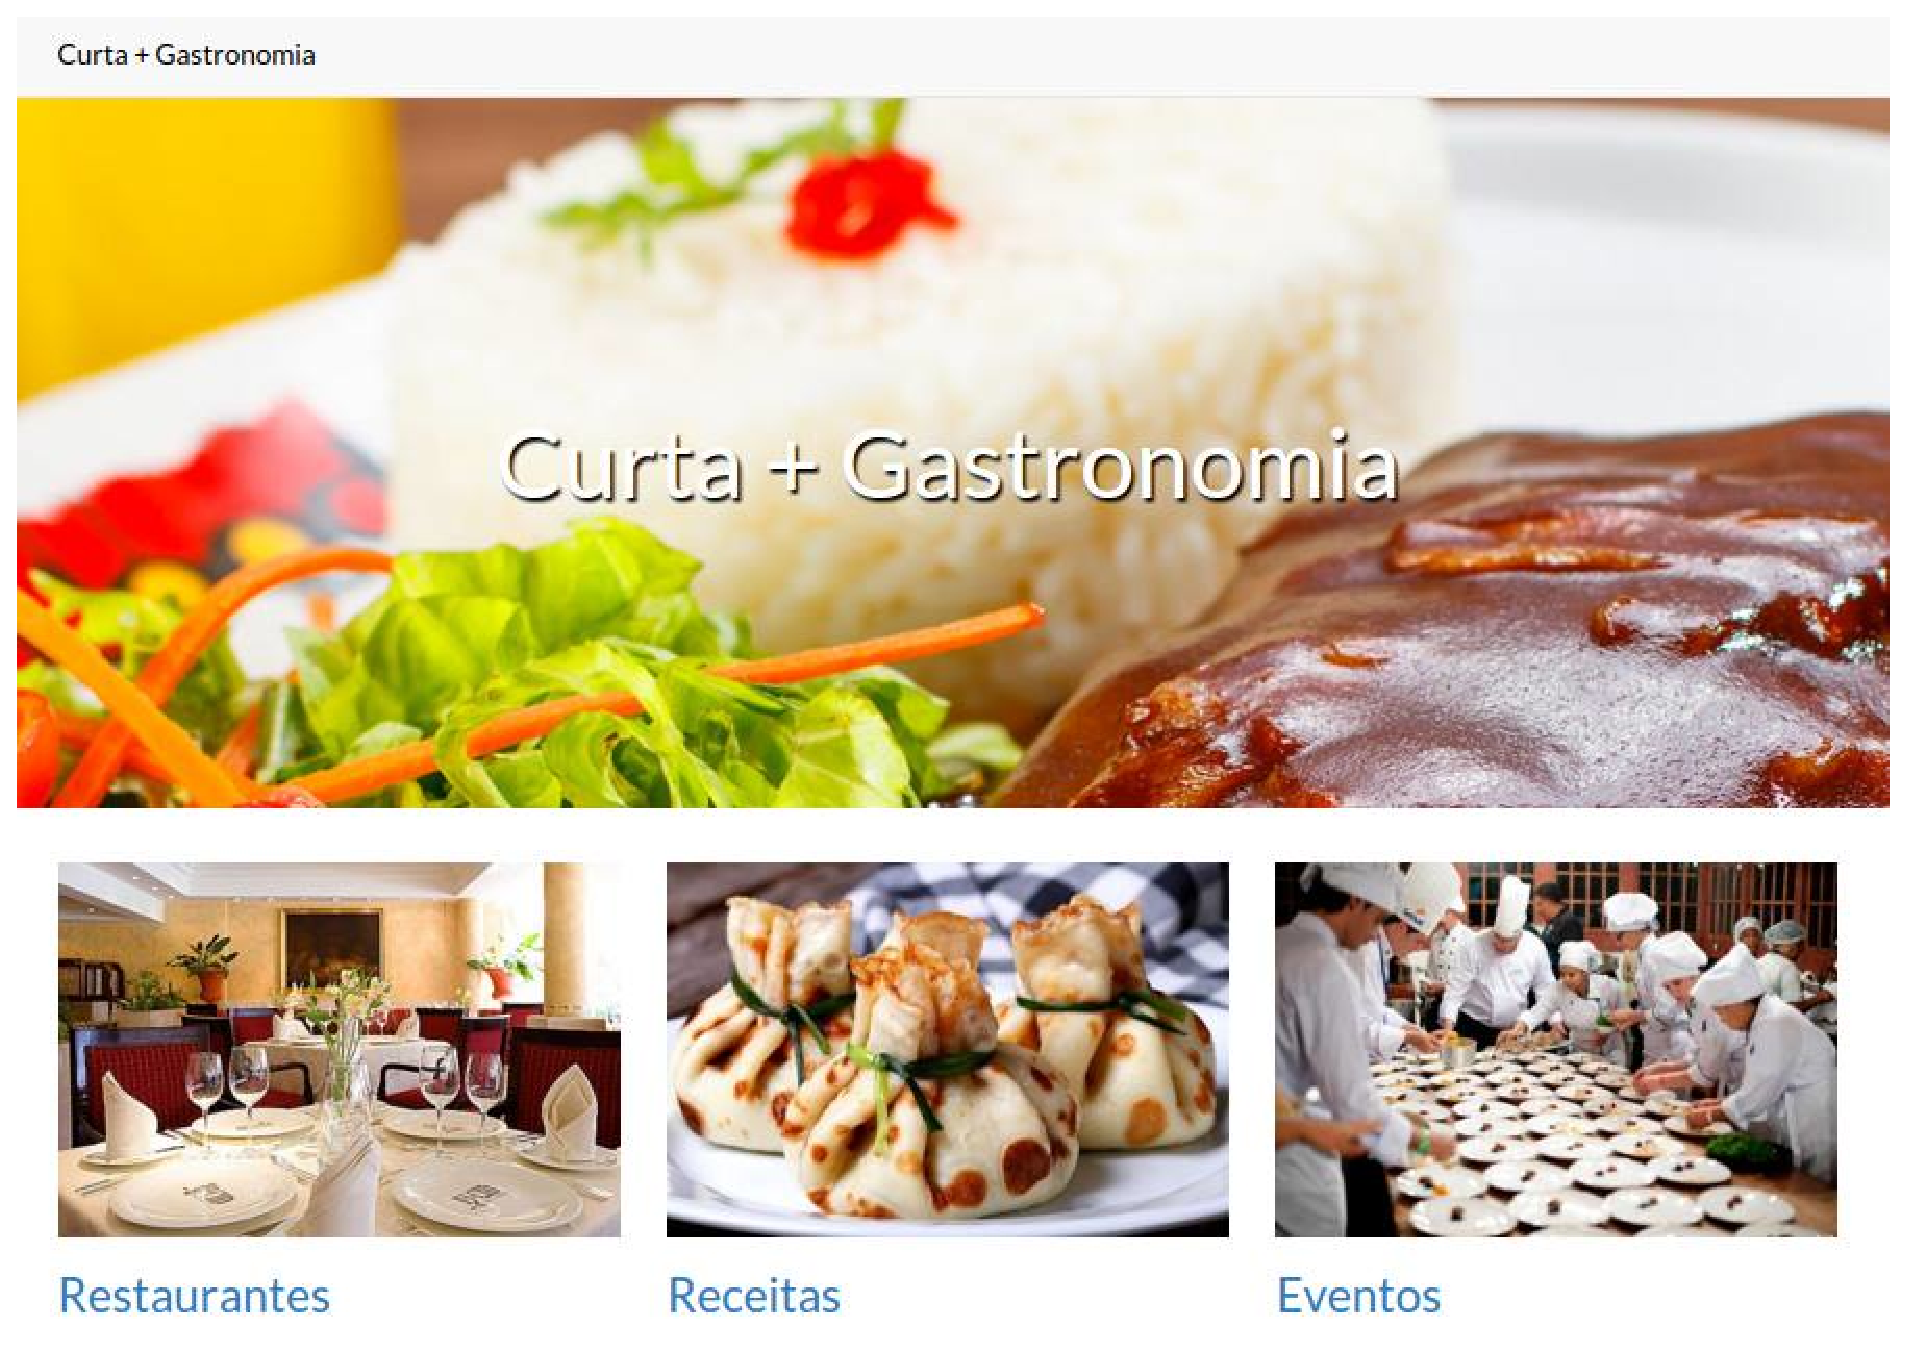
\includegraphics[keepaspectratio,scale=0.3]{figuras/alta_fidelidade/prototipo1.eps}
		\caption{Protótipo Alta Fidelidade}
	\end{center}
\end{figure}

\begin{figure}[H]
	\begin{center}
		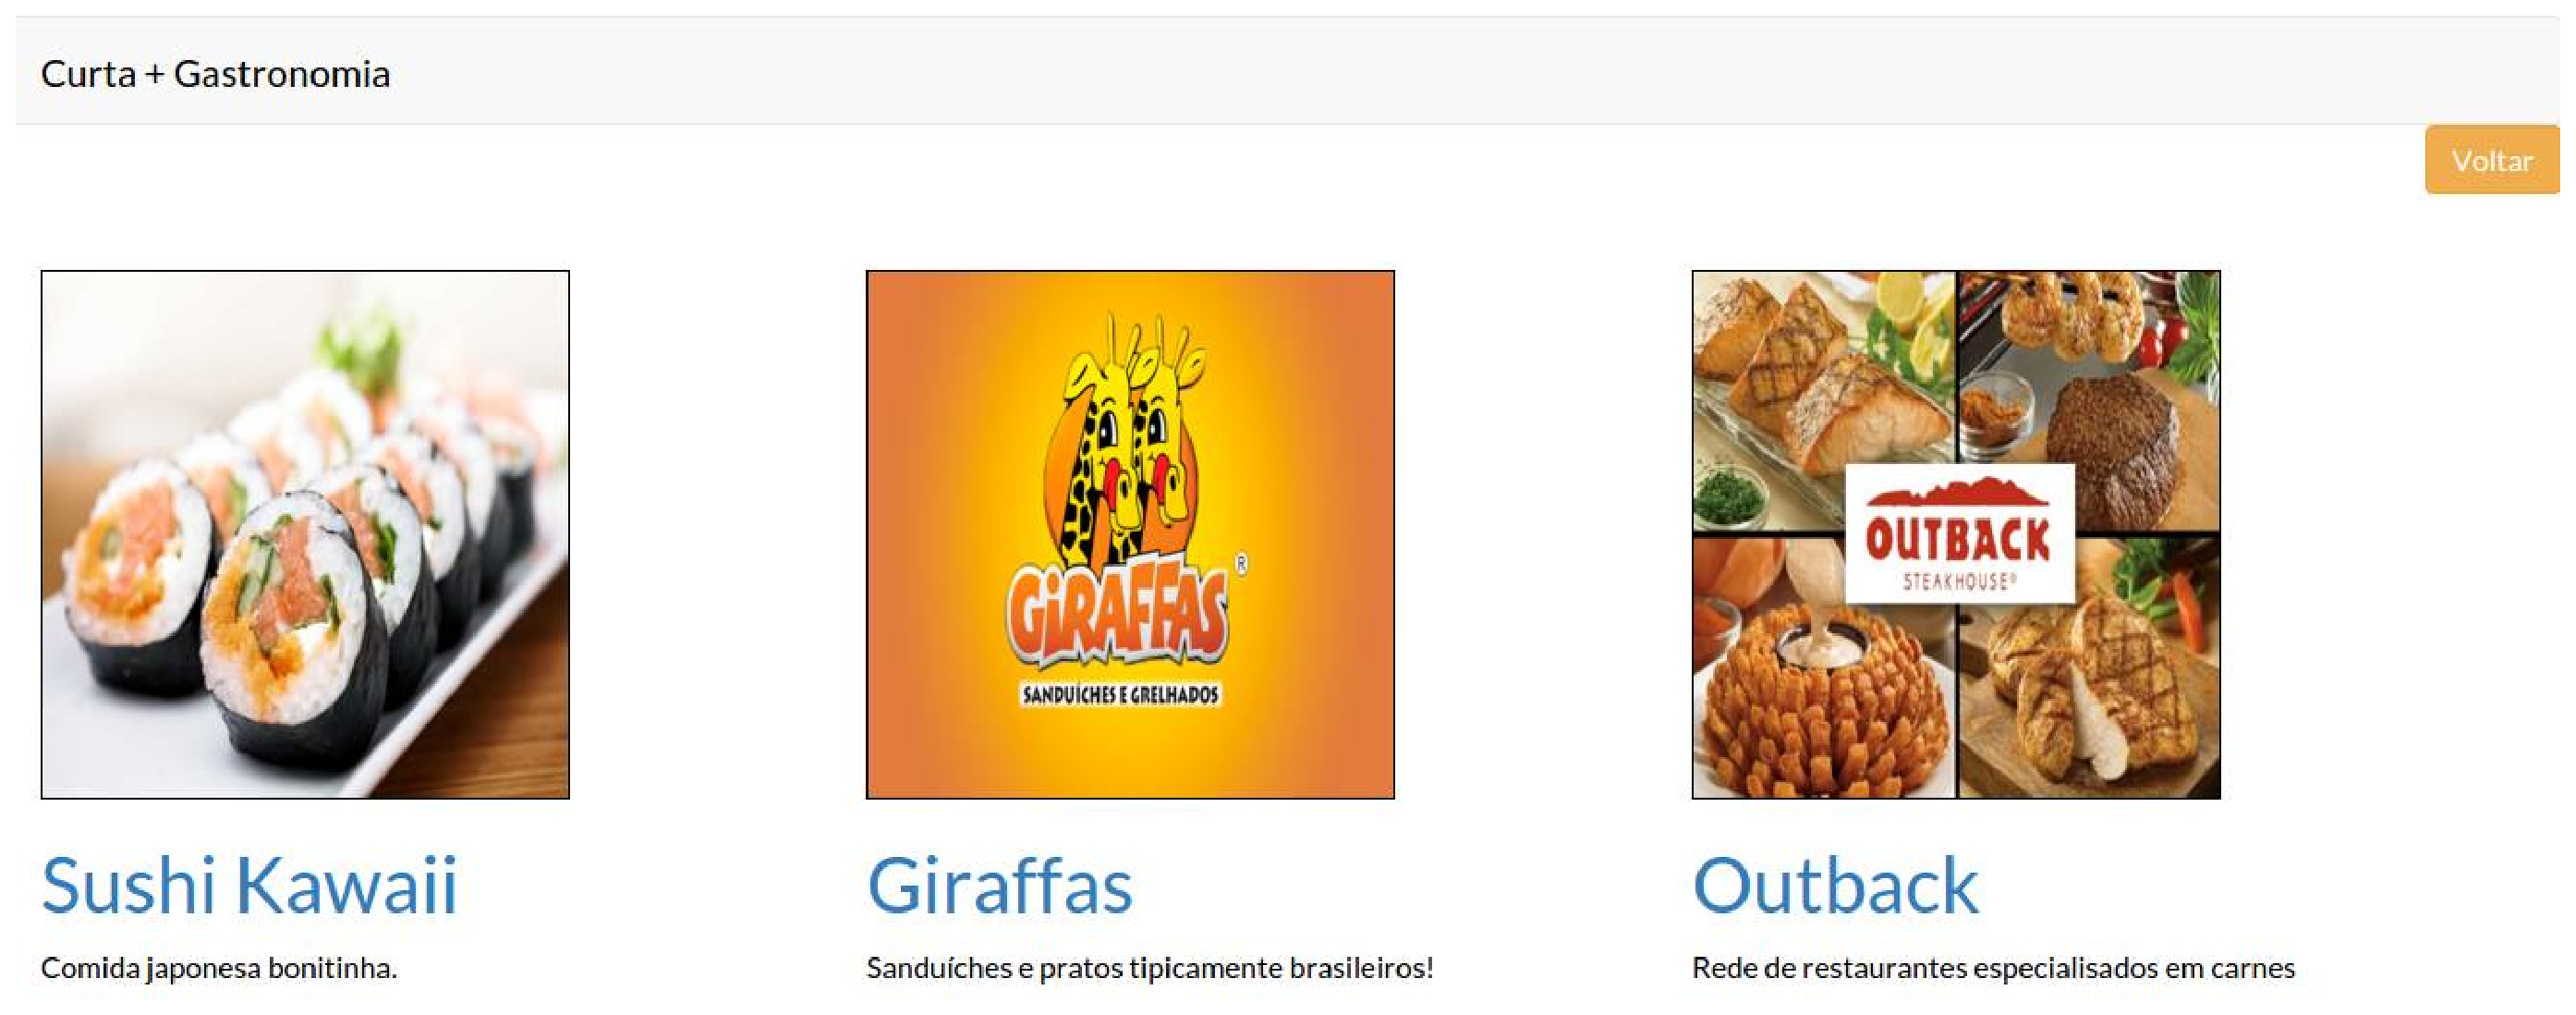
\includegraphics[keepaspectratio,scale=0.3]{figuras/alta_fidelidade/prototipo2.eps}
		\caption{Protótipo Alta Fidelidade}
	\end{center}
\end{figure}

\begin{figure}[H]
	\begin{center}
		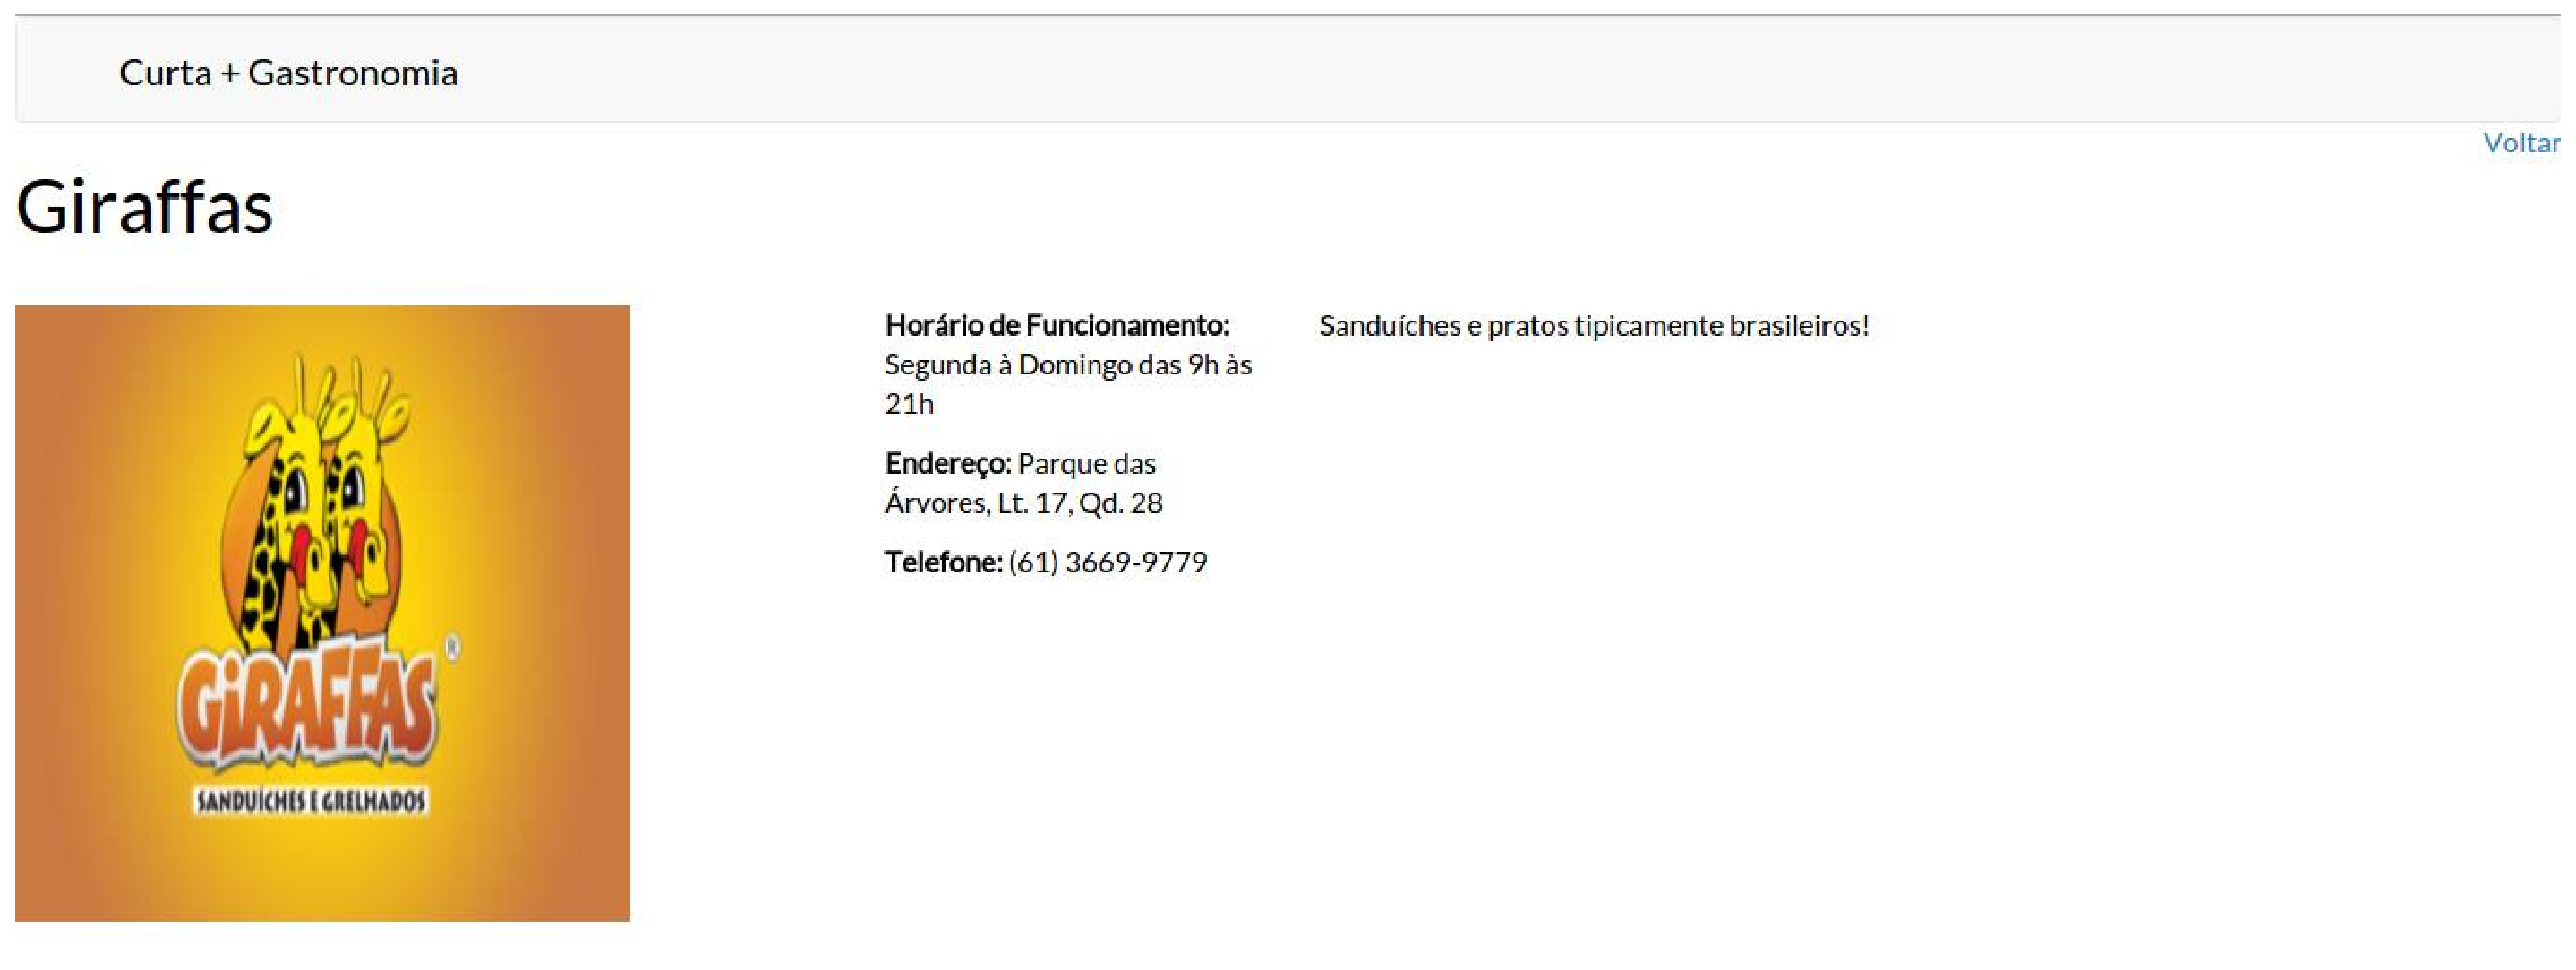
\includegraphics[keepaspectratio,scale=0.3]{figuras/alta_fidelidade/prototipo3.eps}
		\caption{Protótipo Alta Fidelidade}
	\end{center}
\end{figure}

\begin{figure}[H]
	\begin{center}
		\includegraphics[keepaspectratio,scale=0.3]{figuras/alta_fidelidade/prototipo4.eps}
		\caption{Protótipo Alta Fidelidade}
	\end{center}
\end{figure}

\begin{figure}[H]
	\begin{center}
		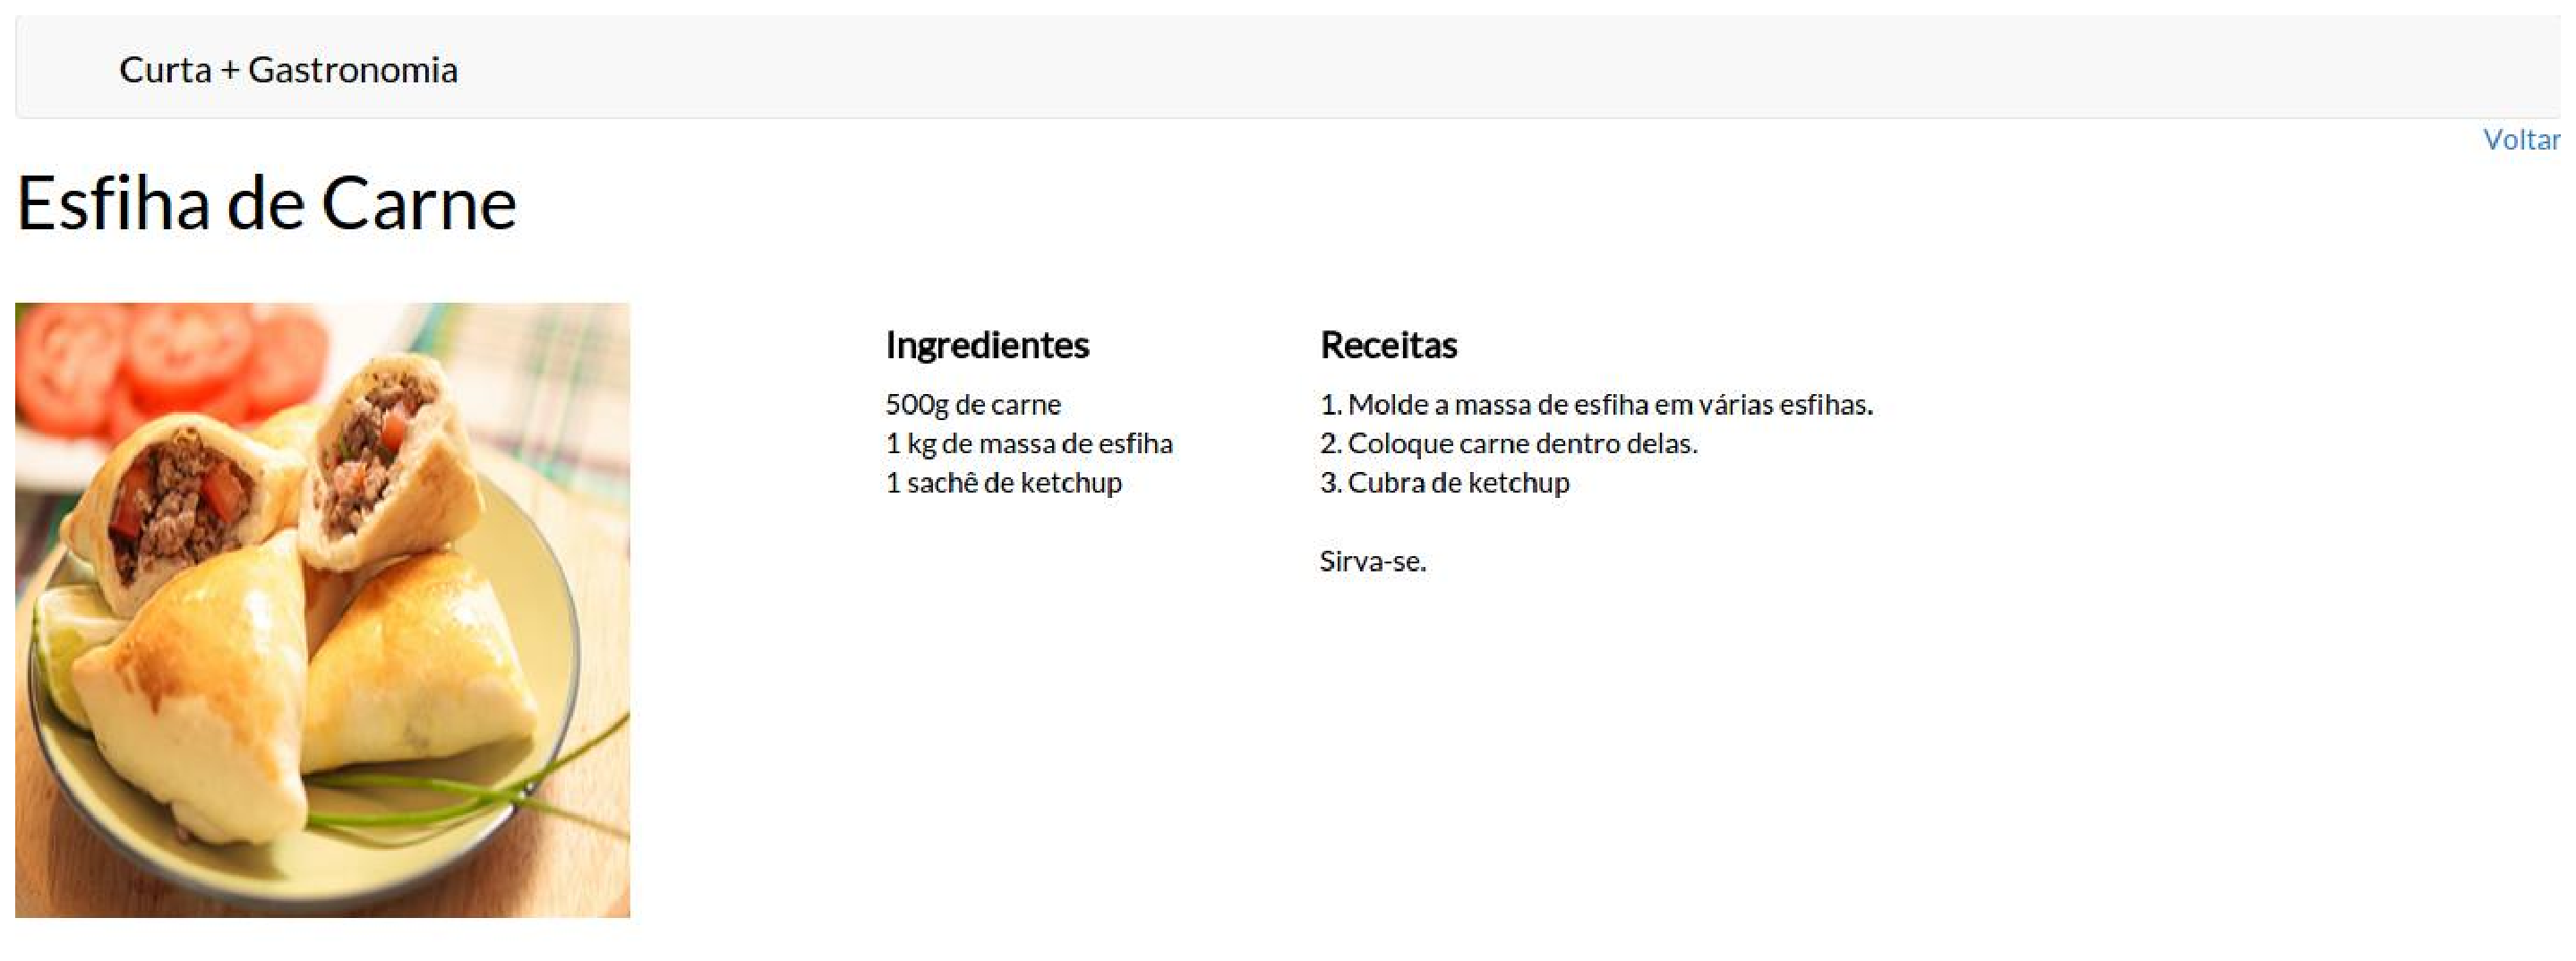
\includegraphics[keepaspectratio,scale=0.3]{figuras/alta_fidelidade/prototipo5.eps}
		\caption{Protótipo Alta Fidelidade}
	\end{center}
\end{figure}

\begin{figure}[H]
	\begin{center}
		\includegraphics[keepaspectratio,scale=0.3]{figuras/alta_fidelidade/prototipo6.eps}
		\caption{Protótipo Alta Fidelidade}
	\end{center}
\end{figure}

\begin{figure}[H]
	\begin{center}
		\includegraphics[keepaspectratio,scale=0.3]{figuras/alta_fidelidade/prototipo7.eps}
		\caption{Protótipo Alta Fidelidade}
	\end{center}
\end{figure}

